% fixture: tikz/tree-foreach-pdftex
% oracle: pdflatex
% tier: T3
% engine: document
% specials: compare
% covers: TikZ trees' child foreach (one child a value of the list, counted among the siblings; several variables, a range, nested, with options and beside plain children)
\documentclass{article}
\usepackage{tikz}
\pagestyle{empty}
\begin{document}
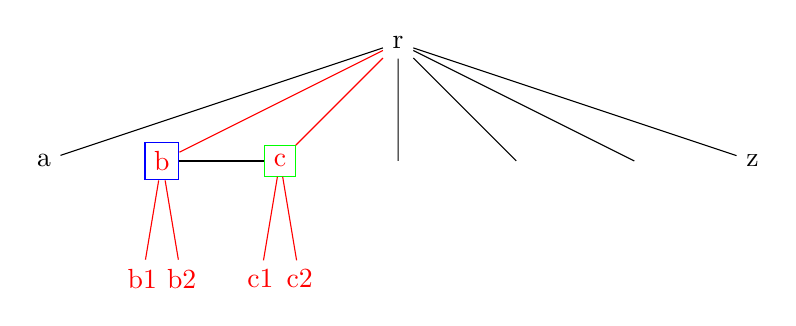
\begin{tikzpicture}[level 2/.style={sibling distance=5mm}]
  \node {r}
    child { node {a} }
    child[red] foreach \x/\c in {b/blue,c/green} { node[draw=\c] (n\x) {\x} child foreach \y in {1,2} { node {\x\y} } }
    child foreach \i in {1,...,3}
    child { node {z} };
  \draw (nb) -- (nc);
\end{tikzpicture}
\end{document}
